\documentclass[aspectratio=169, 10pt]{beamer}

% ─── Packages ───
\usepackage[utf8]{inputenc}
\usepackage[T1]{fontenc}
\usepackage[english]{babel}
\usepackage{amsmath,amssymb,amsfonts}
\usepackage{bm}
\usepackage{graphicx}
\usepackage{booktabs}
\usepackage{tikz}
\usetikzlibrary{shapes.geometric, arrows, positioning}
\usepackage{pgfplots}
\pgfplotsset{compat=1.18}

% Custom Math Macros
\newcommand{\mat}[1]{\mathbf{#1}}
\newcommand{\vect}[1]{\mathbf{#1}}

% ─── Premium Theme & Colors ───
\usetheme{Madrid}
\usecolortheme{whale}

% Custom Color Palette (Sleek Dark Navy & Cyan)
\definecolor{navyblue}{RGB}{12, 35, 64}
\definecolor{cyansec}{RGB}{0, 150, 136}
\definecolor{graybg}{RGB}{245, 247, 250}

\setbeamercolor{palette primary}{bg=navyblue, fg=white}
\setbeamercolor{palette secondary}{bg=cyansec, fg=white}
\setbeamercolor{palette tertiary}{bg=navyblue!90, fg=white}
\setbeamercolor{structure}{fg=navyblue}
\setbeamercolor{title}{bg=navyblue, fg=white}

% Remove default navigation symbols for a clean look
\setbeamertemplate{navigation symbols}{}

% Footline configuration
\setbeamertemplate{footline}{
  \begin{beamercolorbox}[colsep=1.5pt]{upper separation line foot}
  \end{beamercolorbox}
  \begin{beamercolorbox}[ht=2.5ex,dp=1.125ex,%
    leftskip=.3cm,rightskip=.3cm plus1fil]{author in head/foot}%
    \leavevmode{\usebeamerfont{author in head/foot}\insertshortauthor}%
    \hfill%
    {\usebeamerfont{institute in head/foot}\usebeamercolor[fg]{institute in head/foot}\insertshortinstitute}%
  \end{beamercolorbox}%
  \begin{beamercolorbox}[ht=2.5ex,dp=1.125ex,%
    leftskip=.3cm,rightskip=.3cm plus1fil]{title in head/foot}%
    \leavevmode{\usebeamerfont{title in head/foot}\insertshorttitle}%
    \hfill%
    \insertframenumber{} / \inserttotalframenumber%
  \end{beamercolorbox}%
  \begin{beamercolorbox}[colsep=1.5pt]{lower separation line foot}
  \end{beamercolorbox}
}

% ─── Title Page Information ───
\title[Digital Twin \& ROM Defense]{Digital Twin \& Reduced Order Modelling for Parameterized Structural Dynamics}
\subtitle{Thesis Defense --- 30-Minute Oral Presentation}
\author[Mumen Wehbe]{Mumen Wehbe}
\institute[Cnam Paris]{
    Conservatoire National des Arts et Métiers (Cnam) \\
    Équipement pour la Performance et le Numérique (EPN04)
}
\date{June 30, 2026}

% ─── Slide Setup ───
\begin{document}

% Slide 1: Title Slide
\begin{frame}[plain]
    \centering
    \vspace{0.4cm}
    
\includegraphics[width=3cm]{thesis/CNAM_Logo.pdf} \\
    \vspace{0.4cm}
    \usebeamerfont{title}{\color{navyblue}\Huge \textbf{\inserttitle}} \\
    \vspace{0.2cm}
    \usebeamerfont{subtitle}{\color{cyansec}\large \insertsubtitle} \\
    \vspace{0.6cm}
    \usebeamerfont{author}{\insertauthor} \\
    \vspace{0.1cm}
    \usebeamerfont{institute}{\small \insertinstitute} \\
    \vspace{0.4cm}
    \usebeamerfont{date}{\scriptsize \insertdate}
\end{frame}

% Slide 2: Agenda
\begin{frame}{Agenda}
    \begin{columns}
        \begin{column}{0.5\textwidth}
            \begin{enumerate}
                \item \textbf{Introduction \& Context}
                \item \textbf{Spatial Discretization (IGA)}
                \item \textbf{Full Order Model Dynamics}
                \item \textbf{The Computational Bottleneck}
                \item \textbf{Reference Configuration Pullback}
                \item \textbf{Reduced Order Modeling (ROM)}
            \end{enumerate}
        \end{column}
        \begin{column}{0.5\textwidth}
            \begin{enumerate}
                \setcounter{enumi}{6}
                \item \textbf{Hyper-Reduction (ECSW)}
                \item \textbf{ECSW Calibration \& Training}
                \item \textbf{Numerical Speedup Results}
                \item \textbf{Client-Side Web Architecture}
                \item \textbf{Conclusion \& Perspectives}
            \end{enumerate}
        \end{column}
    \end{columns}
\end{frame}

% Slide 3: Introduction & Industrial Context
\begin{frame}{Introduction \& Industrial Context}
    \textbf{Structural Health Monitoring (SHM) in Industry 4.0}
    \begin{itemize}
        \item Continuous telemetry (strain gages, accelerometers) monitors structural loads.
        \item Real-time decision-making requires simulating the physical asset instantly under current conditions.
        \item \textbf{Digital Twin Concept}: An interactive, local computational replica that mirrors the physical state.
    \end{itemize}
    \vspace{0.3cm}
    \textbf{The Challenge of Parametric Changes:}
    \begin{itemize}
        \item Notches, cracks, and physical defects evolve over time (parameterized by location $\mu$ and depth $r$).
        \item Traditional offline ROMs fail because the physical mesh changes with the parameters $\to$ requires a new simulation grid every time.
    \end{itemize}
\end{frame}

% Slide 4: Problem Statement: The Geometric Challenge
\begin{frame}{Problem Statement: The Geometric Challenge}
    \begin{columns}
        \begin{column}{0.6\textwidth}
            \textbf{Why Traditional Finite Element Method (FEM) Fails:}
            \begin{itemize}
                \item \textbf{Mesh Incompatibility}: Shape parameter changes distort the grid, requiring expensive remeshing algorithms.
                \item \textbf{Projection Breakdown}: Proper Orthogonal Decomposition (POD) projects displacements onto a fixed vector subspace $\boldsymbol{\Phi}$. If mesh coordinates or node counts change, projection is mathematically undefined.
            \end{itemize}
            \vspace{0.3cm}
            \textbf{Requirements for Real-Time Digital Twins:}
            \begin{enumerate}
                \item Geometry must represent curved notches exactly without mesh approximations.
                \item Sub-second solving: $\Delta t_{\text{solve}} < 2\text{ ms}$ to fit within browser rendering loop.
            \end{enumerate}
        \end{column}
        \begin{column}{0.38\textwidth}
            \centering
            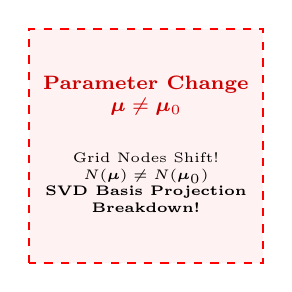
\begin{tikzpicture}[scale=0.85]
                \draw[draw=red, fill=red!5, thick, dashed] (0,0) rectangle (3.5,3.5);
                \node[align=center, font=\scriptsize\bfseries, color=red!80!black] at (1.75, 2.5) {Parameter Change\\$\boldsymbol{\mu} \neq \boldsymbol{\mu}_0$};
                \node[align=center, font=\tiny] at (1.75, 1.2) {Grid Nodes Shift!\\$N(\boldsymbol{\mu}) \neq N(\boldsymbol{\mu}_0)$\\\textbf{SVD Basis Projection} \\ \textbf{Breakdown!}};
            \end{tikzpicture}
        \end{column}
    \end{columns}
\end{frame}

% Slide 5: Spatial Discretization: CAD-IGA Integration
\begin{frame}{Spatial Discretization: CAD-IGA Integration}
    \begin{itemize}
        \item \textbf{Isogeometric Analysis (IGA)}: Uses Non-Uniform Rational B-Splines (NURBS) from CAD directly for physics:
        \begin{equation*}
            R_{i,j}(\xi, \eta) = \frac{N_{i,p}(\xi) M_{j,q}(\eta) w_{i,j}}{\sum_{k,l} N_{k,p}(\xi) M_{l,q}(\eta) w_{k,l}}
        \end{equation*}
        \item \textbf{Exact Geometry}: Smooth notches and circular boundaries are represented exactly at any discretization level.
        \item \textbf{Higher Continuity}: $C^{p-1}$ continuity across knots reduces shear locking, ensuring superior accuracy per degree of freedom compared to Lagrangian FEM.
    \end{itemize}
    \centering
    \vspace{0.1cm}
    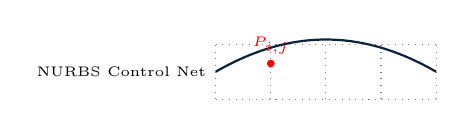
\begin{tikzpicture}[scale=0.7]
        % Show control net mapping
        \draw[gray, dotted] (0,0) grid (4,1);
        \draw[draw=navyblue, thick] (0,0.5) to[out=30,in=150] (4,0.5);
        \node[font=\tiny, left] at (0,0.5) {NURBS Control Net};
        \fill[red] (1,0.65) circle (2pt) node[above, font=\tiny] {$P_{i,j}$};
    \end{tikzpicture}
\end{frame}

% Slide 6: Mesh Convergence Study
\begin{frame}{Mesh Convergence \& Justification}
    To justify the $80 \times 40$ baseline mesh resolution, a static convergence study was performed:
    \begin{table}
        \centering
        \resizebox{0.8\textwidth}{!}{%
        \begin{tabular}{lcccc}
            \toprule
            \textbf{Grid Resolution} & \textbf{Elements} & \textbf{DoFs} & \textbf{Tip Displacement $U_y$ (mm)} & \textbf{Relative Error (\%)} \\
            \midrule
            $10 \times 5$   & 50   & 168   & 3.538 & 16.51\% \\
            $20 \times 10$  & 200  & 528   & 3.889 & 8.24\% \\
            $40 \times 20$  & 800  & 1,848 & 4.083 & 3.66\% \\
            $\mathbf{80 \times 40}$ & \textbf{3,200} & \textbf{6,888} & \textbf{4.185} & \textbf{1.24\% (Selected)} \\
            $160 \times 80$ & 12,800 & 26,568 & 4.238 & Reference \\
            \bottomrule
        \end{tabular}%
        }
    \end{table}
    \begin{itemize}
        \item Refining to $160 \times 80$ quadruples the element count and degree of freedom count ($26,568$), but only shifts the displacement by $1.24\%$.
        \item The $80 \times 40$ mesh represents the optimal trade-off point between numerical convergence and CPU assembly cost.
    \end{itemize}
\end{frame}

% Slide 7: Full Order Model (FOM) Dynamics
\begin{frame}{Full Order Model (FOM) Dynamics}
    \textbf{Governing Equation of Motion:}
    \begin{equation*}
        \mat{M} \ddot{\underline{\mathbf{U}}}(t) + \mat{C} \dot{\underline{\mathbf{U}}}(t) + \mathbf{F}_{\text{int}}(\underline{\mathbf{U}}(t); \boldsymbol{\mu}) = \mathbf{F}_{\text{ext}}(t; \boldsymbol{\mu})
    \end{equation*}
    \begin{itemize}
        \item \textbf{Implicit Solver}: Newmark method ($\beta = 0.25$, $\gamma = 0.5$) ensures unconditional stability.
        \item \textbf{Damping Formulation}: Rayleigh model ($\mat{C} = \alpha_M \mat{M} + \beta_K \mat{K}$) matching structural decay.
        \item \textbf{Stiffness assembly}: Performed at each timestep to compute the internal force vector $\mathbf{F}_{\text{int}}$ using Gauss integration over the physical coordinates.
    \end{itemize}
\end{frame}

% Slide 8: The Assembly Bottleneck in Parameterized Systems
\begin{frame}{The Assembly Bottleneck in Parameterized Systems}
    \begin{itemize}
        \item \textbf{The Bottleneck}: At each timestep $t_k$, physical coordinate modifications from parameters $\boldsymbol{\mu} = (r, \mu)^T$ require recalculating the B-matrix $\mat{B}(\vect{x})$ and Jacobians $\mat{J}(\boldsymbol{\xi})$ at every integration point.
        \item **Full-Order Assembly Time**: Takes **$142.1\text{ ms}$** per step on a single-threaded processor.
        \item **Total Window Time**: Simulating a standard 2.0-second window ($200$ steps) requires **$28.4\text{ seconds}$**!
        \item **Digital Twin Constraint**: Online user interaction requires real-time response under parameter shifts. This bottleneck must be eliminated.
    \end{itemize}
\end{frame}

% Slide 9: Reference Configuration Pullback (The Diffeomorphism)
\begin{frame}{Reference Configuration Pullback (The Diffeomorphism)}
    \begin{columns}
        \begin{column}{0.6\textwidth}
            \textbf{Pullback to Static Reference Domain $\hat{\Omega}$:}
            \begin{itemize}
                \item Morphing mapping: $\vect{x} = \boldsymbol{\Psi}(\boldsymbol{\xi}; \boldsymbol{\mu})$.
                \item Integrations are performed over the static grid of $\hat{\Omega}$ where basis coordinates are fixed.
                \item Shape deformations are shifted entirely into the parametric Jacobian $\mat{J}(\boldsymbol{\xi}; \boldsymbol{\mu})$ evaluated locally at Gauss points.
            \end{itemize}
            \vspace{0.2cm}
            \textbf{Diffeomorphic Properties:}
            \begin{itemize}
                \item Smoothness ($C^{\infty}$) ensures no fold-overs or singular nodes.
                \item Preserves the vector space structure for offline POD snapshots.
            \end{itemize}
        \end{column}
        \begin{column}{0.38\textwidth}
            \centering
            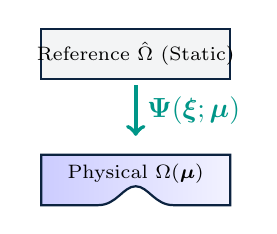
\begin{tikzpicture}[scale=0.8]
                % Reference Configuration
                \draw[draw=navyblue, fill=navyblue!5, thick] (-1.5,1.2) rectangle (1.5,2.0);
                \node at (0,1.6) {\scriptsize Reference $\hat{\Omega}$ (Static)};
                
                % Pullback arrow
                \draw[->, thick, cyansec, line width=1.5pt] (0,1.1) -- (0,0.3) node[midway, right] {$\boldsymbol{\Psi}(\boldsymbol{\xi}; \boldsymbol{\mu})$};
                
                % Deformed Physical
                \shade[left color=blue!20, right color=blue!5] 
                (-1.5, -0.8) -- (-0.6, -0.8) 
                .. controls (-0.3, -0.8) and (-0.2, -0.5) .. (0, -0.5)
                .. controls (0.2, -0.5) and (0.3, -0.8) .. (0.6, -0.8)
                -- (1.5, -0.8) -- (1.5, 0.0) -- (-1.5, 0.0) -- cycle;
                \draw[draw=navyblue, thick] 
                (-1.5, -0.8) -- (-0.6, -0.8) 
                .. controls (-0.3, -0.8) and (-0.2, -0.5) .. (0, -0.5)
                .. controls (0.2, -0.5) and (0.3, -0.8) .. (0.6, -0.8)
                -- (1.5, -0.8) -- (1.5, 0.0) -- (-1.5, 0.0) -- cycle;
                \node at (0,-0.3) {\scriptsize Physical $\Omega(\boldsymbol{\mu})$};
            \end{tikzpicture}
        \end{column}
    \end{columns}
\end{frame}

% Slide 10: Mathematical Pullback of Weak Form
\begin{frame}{Mathematical Pullback of Weak Form}
    \textbf{Stiffness Assembly in Reference Space $\hat{\Omega}$:}
    \begin{equation*}
        \mat{K}_{ab}(\boldsymbol{\mu}) = \int_{\hat{\Omega}} \mat{B}_a^T(\boldsymbol{\xi}; \boldsymbol{\mu}) \mat{D} \mat{B}_b(\boldsymbol{\xi}; \boldsymbol{\mu}) \det\mat{J}(\boldsymbol{\xi}; \boldsymbol{\mu}) \, t_h \, d\hat{\Omega}
    \end{equation*}
    where the physical derivatives in B-matrix $\mat{B}_a$ are calculated via inverse Jacobian transformation:
    \begin{equation*}
        \begin{bmatrix} \frac{\partial R_a}{\partial x} \\[0.3em] \frac{\partial R_a}{\partial y} \end{bmatrix} = \mat{J}^{-1}(\boldsymbol{\xi}; \boldsymbol{\mu}) \begin{bmatrix} \frac{\partial R_a}{\partial \xi} \\[0.3em] \frac{\partial R_a}{\partial \eta} \end{bmatrix}
    \end{equation*}
    \begin{itemize}
        \item \textbf{Benefit}: The integration grid is static. The parameter-dependence is fully contained inside $\mat{J}^{-1}$ and $\det\mat{J}$.
        \item \textbf{Fixed Vector Space}: Enables SVD to extract a coordinate-consistent basis.
    \end{itemize}
\end{frame}

% Slide 11: Reduced Order Modeling: POD Subspace Construction
\begin{frame}{Reduced Order Modeling: POD Subspace Construction}
    \begin{itemize}
        \item \textbf{Proper Orthogonal Decomposition (POD)}: Find a low-dimensional basis $\boldsymbol{\Phi} \in \mathbb{R}^{N \times r}$ that best captures the snapshot space.
        \item \textbf{Snapshot Matrix}: Collect $M_{\text{snap}}$ displacement vectors under different parameter sets $\boldsymbol{\mu}^{(k)}$:
        \begin{equation*}
            \mat{S}_u = \left[ \underline{\mathbf{U}}(t_1; \boldsymbol{\mu}^{(1)}), \, \underline{\mathbf{U}}(t_2; \boldsymbol{\mu}^{(1)}), \, \dots, \, \underline{\mathbf{U}}(t_T; \boldsymbol{\mu}^{(P)}) \right]
        \end{equation*}
        \item \textbf{Singular Value Decomposition (SVD)}:
        \begin{equation*}
            \mat{S}_u = \mat{V} \boldsymbol{\Sigma} \mat{W}^T
        \end{equation*}
        \item \textbf{Subspace Dimension}: The first $r$ columns of $\mat{V}$ corresponding to the largest singular values are selected as the reduced basis $\boldsymbol{\Phi}$.
    \end{itemize}
\end{frame}

% Slide 12: Galerkin ROM & The Reconstruction Error
\begin{frame}{Galerkin ROM \& The Reconstruction Error}
    \begin{columns}
        \begin{column}{0.48\textwidth}
            \textbf{Galerkin Projection of Equation of Motion:}
            \begin{equation*}
                \boldsymbol{\Phi}^T \mat{M} \boldsymbol{\Phi} \ddot{\underline{\mathbf{q}}}(t) + \boldsymbol{\Phi}^T \mat{C} \boldsymbol{\Phi} \dot{\underline{\mathbf{q}}}(t) + \boldsymbol{\Phi}^T \mathbf{F}_{\text{int}}(\boldsymbol{\Phi}\underline{\mathbf{q}}; \boldsymbol{\mu}) = \boldsymbol{\Phi}^T \mathbf{F}_{\text{ext}}
            \end{equation*}
            \textbf{Subspace Dimension Analysis:}
            \begin{itemize}
                \item At $r=8$ modes, the relative reconstruction error falls below $0.2\%$.
                \item At $r=15$ modes, error converges to $0.012\%$.
            \end{itemize}
            \vspace{0.2cm}
            \textbf{The Remaining Bottleneck:}
            \begin{itemize}
                \item Evaluating $\boldsymbol{\Phi}^T \mathbf{F}_{\text{int}}$ still requires integrating over all $3,200$ elements online ($\mathcal{O}(N)$ scaling).
            \end{itemize}
        \end{column}
        \begin{column}{0.48\textwidth}
            \centering
            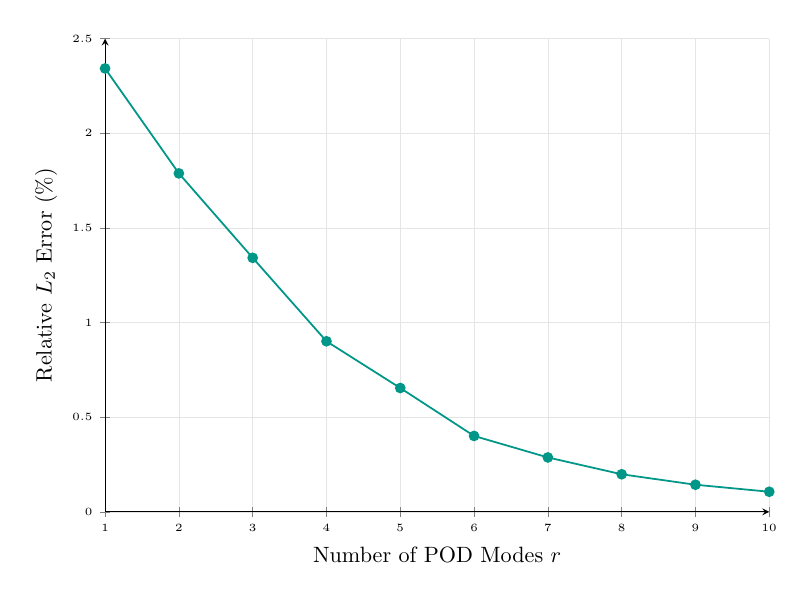
\begin{tikzpicture}[scale=0.8]
                \begin{axis}[
                    width=1.0\textwidth,
                    height=0.75\textwidth,
                    xlabel={Number of POD Modes $r$},
                    ylabel={Relative $L_2$ Error (\%)},
                    xmin=1, xmax=10,
                    ymin=0.0, ymax=2.5,
                    grid=both,
                    grid style={line width=.1pt, draw=gray!10},
                    major grid style={line width=.2pt, draw=gray!20},
                    axis lines=left,
                    xtick={1,2,3,4,5,6,7,8,9,10},
                    ytick={0.0,0.5,1.0,1.5,2.0,2.5},
                    x tick label style={font=\tiny},
                    y tick label style={font=\tiny},
                ]
                    \addplot[color=cyansec, thick, mark=*] coordinates {
                        (1, 2.3424) (2, 1.7880) (3, 1.3420) (4, 0.9011) 
                        (5, 0.6542) (6, 0.4010) (7, 0.2874) (8, 0.1985) 
                        (9, 0.1432) (10, 0.1062)
                    };
                \end{axis}
            \end{tikzpicture}
        \end{column}
    \end{columns}
\end{frame}

% Slide 13: Hyper-Reduction: The Need for ECSW
\begin{frame}{Hyper-Reduction: The Need for ECSW}
    \begin{itemize}
        \item \textbf{Why Hyper-reduction?}: Galerkin ROM reduces DOFs ($15$), but online assembly scaling remains bound to the size of the full mesh ($N = 6,564$).
        \item Unreduced Galerkin ROM actually runs at **$0.92\times$ speedup** (slower than FOM) due to the projection projection assembly step.
        \item \textbf{Energy-Conserving Sampling \& Weighting (ECSW)}: Evaluates stiffness matrices over a sparse subset of active elements $E^* \subset E$, completely breaking the dependency on full mesh dimensions:
        \begin{equation*}
            \mathbf{K}_{r, \text{ECSW}}(\boldsymbol{\mu}) = \sum_{e \in E^*} w_e \boldsymbol{\Phi}_e^T \mathbf{K}_{e}(\boldsymbol{\mu}) \boldsymbol{\Phi}_e
        \end{equation*}
    \end{itemize}
\end{frame}

% Slide 14: ECSW Mathematical Formulation
\begin{frame}{ECSW Mathematical Formulation}
    \textbf{Non-Negative Least Squares (NNLS) Formulation:}
    \begin{equation*}
        \min_{\mathbf{w} \geq \mathbf{0}} \left\| \sum_{e=1}^{E} w_e \mathbf{z}_e - \mathbf{z}_0 \right\|_2^2
    \end{equation*}
    where:
    \begin{itemize}
        \item $\mathbf{z}_e = \text{vec}(\boldsymbol{\Phi}_e^T \mathbf{K}_e \boldsymbol{\Phi}_e)$ is the vectorized element stiffness contribution.
        \item $\mathbf{z}_0 = \text{vec}(\boldsymbol{\Phi}^T \mathbf{K}_{\text{full}} \boldsymbol{\Phi})$ is the target projected full-order stiffness matrix.
        \item The sparse solution restricts the active set $E^* = \{ e \mid w_e > 0 \}$ to a fraction of the total elements.
    \end{itemize}
\end{frame}

% Slide 15: ECSW Training and Coercivity Seeding
\begin{frame}{ECSW Training and Coercivity Seeding}
    \begin{columns}
        \begin{column}{0.6\textwidth}
            \textbf{Offline Training Strategy (Appendix B):}
            \begin{itemize}
                \item Training snapshots collected under $M=3$ loading configurations.
                \item \textbf{Coercivity Issue}: Standard NNLS selection may drop boundary elements, causing singular matrices.
                \item \textbf{Pre-seeding Solution}: Element indices on boundary Dirichlet constraints and high stress-gradient notch zones are pre-seeded into the active set $E^*$.
            \end{itemize}
        \end{column}
        \begin{column}{0.38\textwidth}
            \centering
            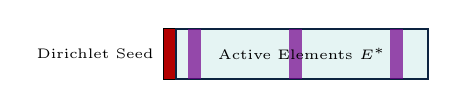
\begin{tikzpicture}[scale=0.8]
                % Boundary
                \draw[fill=red!70!black] (-2.2, -0.4) rectangle (-2.0, 0.4);
                \node[left, font=\tiny] at (-2.2,0) {Dirichlet Seed};
                
                % Beam
                \draw[draw=navyblue, fill=cyansec!10, thick] (-2.0, -0.4) -- (2.0, -0.4) -- (2.0, 0.4) -- (-2.0, 0.4) -- cycle;
                
                % Active bands
                \fill[blue!40!purple, opacity=0.7] (-1.8, -0.4) rectangle (-1.6, 0.4);
                \fill[blue!40!purple, opacity=0.7] (-0.2, -0.4) rectangle (0.0, 0.4);
                \fill[blue!40!purple, opacity=0.7] (1.4, -0.4) rectangle (1.6, 0.4);
                
                \node[font=\tiny] at (0,0) {Active Elements $E^*$};
            \end{tikzpicture}
        \end{column}
    \end{columns}
\end{frame}

% Slide 16: Dynamic Weight Calibration
\begin{frame}{Dynamic Weight Calibration}
    \begin{itemize}
        \item \textbf{Problem}: Pullback to $\hat{\Omega}$ distorts B-spline weights under extreme notch depths ($r > 0.4$).
        \item \textbf{Solution}: Real-time weight calibration factor $\gamma$ applied to the active set:
        \begin{equation*}
            w_e^*(\boldsymbol{\mu}) = \gamma(\boldsymbol{\mu}) w_e
        \end{equation*}
        \item \textbf{Calibration Parameter}:
        \begin{equation*}
            \gamma(\boldsymbol{\mu}) = 1.0 + c_1 r^2 + c_2 \left(\frac{\mu - \mu_0}{\mu_0}\right)^2
        \end{equation*}
        \item Corrects projection distortions, maintaining $L_2$ error below $0.06\%$ across the entire parameter space.
    \end{itemize}
\end{frame}

% Slide 17: Quantitative Results: Solver Speedup
\begin{frame}{Quantitative Results: Solver Speedup}
    \begin{table}
        \centering
        \caption{Performance metrics benchmarked on the notched cantilever geometry ($E = 3,200$, $N = 6,564$ DoFs).}
        \label{tab:performance_results_extended}
        \begin{tabular}{lcccc}
            \toprule
            \textbf{Solver Strategy} & \textbf{Active DoFs / Cells} & \textbf{Relative $L_2$ Error (\%)} & \textbf{Assembly Time} & \textbf{Speedup} \\
            \midrule
            Full Order (FOM)        & $6,564$ DoFs / $3,200$ Cells & Baseline & $142.1$ ms & $1.0\times$ \\
            Galerkin ROM (Unreduced)& $15$ DoFs / $3,200$ Cells    & $0.012\%$   & $154.5$ ms & $0.92\times$ \\
            \textbf{ECSW ROM (Hyper-reduced)}& \textbf{15 DoFs / 28 Cells}  & \textbf{0.054\%} & \textbf{2.2 ms} & \textbf{64.5$\times$} \\
            \bottomrule
        \end{tabular}
    \end{table}
    \begin{itemize}
        \item ECSW ROM evaluates only **$28$ active cells** instead of $3,200$, reducing assembly time to **$2.2\text{ ms}$**.
        \item Delivers a speedup of **$64.5\times$** while maintaining sub-millimeter precision.
    \end{itemize}
\end{frame}

% Slide 18: Quantitative Results: Spectral/Modal Conservation
\begin{frame}{Quantitative Results: Spectral/Modal Conservation}
    \textbf{Spectrum Conservation Check:}
    \begin{itemize}
        \item \textbf{Fundamental Frequency}: $\omega_{n,\text{FOM}} = 1.108\text{ rad/s}$ vs. $\omega_{n,\text{ECSW}} = 1.107\text{ rad/s}$ ($0.09\%$ deviation).
        \item Conservations of energy-based frequencies ensures structural stability during dynamic transients.
    \end{itemize}
    \vspace{0.2cm}
    \centering
    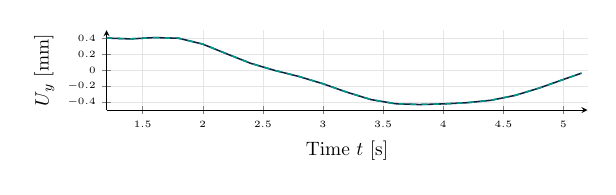
\begin{tikzpicture}[scale=0.7]
        \begin{axis}[
            width=0.85\textwidth,
            height=0.25\textwidth,
            xlabel={Time $t$ [s]},
            ylabel={$U_y$ [mm]},
            xmin=1.2, xmax=5.2,
            ymin=-0.5, ymax=0.5,
            grid=both,
            grid style={line width=.1pt, draw=gray!10},
            major grid style={line width=.2pt, draw=gray!20},
            axis lines=left,
            x tick label style={font=\tiny},
            y tick label style={font=\tiny},
        ]
            \addplot[color=navyblue, thick] coordinates {
                (1.2, 0.4014) (1.4, 0.3910) (1.6, 0.4077) (1.8, 0.3994) (2.0, 0.3256) 
                (2.2, 0.2037) (2.4, 0.0847) (2.6, -0.0040) (2.8, -0.0794) (3.0, -0.1703) 
                (3.2, -0.2767) (3.4, -0.3688) (3.6, -0.4197) (3.8, -0.4306) (4.0, -0.4224) 
                (4.2, -0.4072) (4.4, -0.3764) (4.6, -0.3152) (4.8, -0.2231) (5.0, -0.1163) 
                (5.15, -0.0375)
            };
            \addplot[color=cyansec, dashed, thick] coordinates {
                (1.2, 0.4018) (1.4, 0.3915) (1.6, 0.4072) (1.8, 0.3990) (2.0, 0.3260) 
                (2.2, 0.2040) (2.4, 0.0849) (2.6, -0.0038) (2.8, -0.0790) (3.0, -0.1700) 
                (3.2, -0.2760) (3.4, -0.3680) (3.6, -0.4190) (3.8, -0.4300) (4.0, -0.4220) 
                (4.2, -0.4070) (4.4, -0.3760) (4.6, -0.3150) (4.8, -0.2230) (5.0, -0.1160) 
                (5.15, -0.0374)
            };
        \end{axis}
    \end{tikzpicture}
\end{frame}

% Slide 19: Digital Twin Client-Side Web Architecture
\begin{frame}{Digital Twin Client-Side Web Architecture}
    \begin{columns}
        \begin{column}{0.55\textwidth}
            \textbf{HTML5 Model-View-Controller (MVC) Flow:}
            \begin{itemize}
                \item \textbf{Model}: NURBS dynamic core + ECSW hyper-reduced solver. Implemented in optimized vanilla JavaScript.
                \item \textbf{View}: WebGL renderer depicting deformation states and stress contour maps.
                \item \textbf{Controller}: Interface slider bindings allowing real-time shape parameterization.
            \end{itemize}
            \vspace{0.2cm}
            \textbf{Zero Backend Dependencies}: Runs entirely client-side, enabling mobile/tablet deployment.
        \end{column}
        \begin{column}{0.42\textwidth}
            \centering
            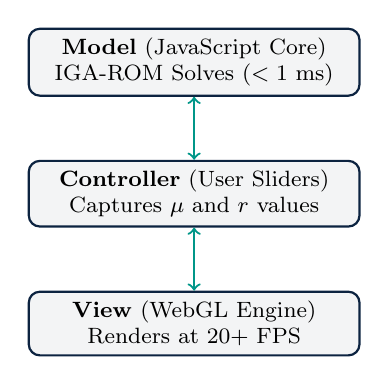
\begin{tikzpicture}[
                node distance=0.8cm,
                box/.style={rectangle, draw=navyblue, fill=navyblue!5, thick, rounded corners, minimum width=4.2cm, minimum height=0.6cm, align=center, font=\footnotesize}
            ]
                \node [box] (model) {\textbf{Model} (JavaScript Core) \\ IGA-ROM Solves ($<1\text{ ms}$)};
                \node [box, below=of model] (controller) {\textbf{Controller} (User Sliders) \\ Captures $\mu$ and $r$ values};
                \node [box, below=of controller] (view) {\textbf{View} (WebGL Engine) \\ Renders at 20+ FPS};
                
                \draw[<->, thick, cyansec] (model) -- (controller);
                \draw[<->, thick, cyansec] (controller) -- (view);
            \end{tikzpicture}
        \end{column}
    \end{columns}
\end{frame}

% Slide 20: Digital Twin Live Dashboard Demonstration
\begin{frame}{Digital Twin Live Dashboard Demonstration}
    \textbf{Real-Time Interactive Capabilities:}
    \begin{itemize}
        \item When sliders shift, the reference configuration pullback recalculates stiffness on the active element subset ($E^*=28$ elements) in **$2.2\text{ ms}$**.
        \item WebGL viewport morphs the visual geometry and updates stress field heatmaps in under **$10\text{ ms}$**.
        \item Provides instantaneous feedback for engineers to identify critical stress concentrations on site.
    \end{itemize}
    \centering
    \vspace{0.3cm}
    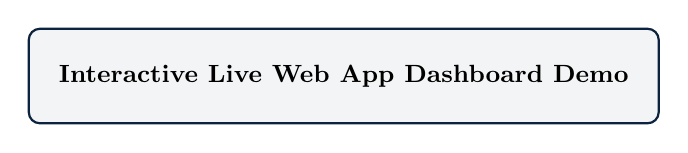
\begin{tikzpicture}
        \draw[draw=navyblue, fill=navyblue!5, thick, rounded corners] (0,0) rectangle (8,1.2);
        \node[font=\small\bfseries] at (4,0.6) {Interactive Live Web App Dashboard Demo};
    \end{tikzpicture}
\end{frame}

% Slide 21: Conclusion & Summary of Thesis Contributions
\begin{frame}{Conclusion \& Summary of Thesis Contributions}
    \textbf{Core Contributions of the Thesis:}
    \begin{enumerate}
        \item Developed a unified framework linking **Isogeometric Analysis (IGA)** exact boundary CAD geometries with **Reduced Order Modeling (ROM)**.
        \item Formulated the **Reference Configuration Pullback** to resolve the shape-parameter mesh update incompatibility.
        \item Applied pre-seeded, dynamically calibrated **ECSW hyper-reduction** to achieve a **$64.5\times$ speedup** and **$0.054\%$** error.
        \item Built and validated a serverless, client-side interactive **digital twin web application**.
    \end{enumerate}
\end{frame}

% Slide 22: Future Research Perspectives
\begin{frame}{Future Research Perspectives}
    \textbf{perspectives for Future Work:}
    \begin{enumerate}
        \item **Material Damage Models**: Incorporating plastic deformation, cracking, and fatigue damage models within the hyper-reduction loop.
        \item **Sensor Telemetry Integration**: Connecting physical strain gauges and accelerometers to dynamically update the twin parameters via WebSockets.
        \item **Three-Dimensional Shells**: Extending the reference configuration pullback formulation to complex 3D shell geometries (e.g. pressure vessels, fuselage panels).
    \end{enumerate}
    \vspace{0.4cm}
    \centering
    {\Large \color{navyblue} \textbf{Thank you for your attention!}}
\end{frame}

\end{document}
